% -- Encoding UTF-8 without BOM
% -- XeLaTeX => PDF (BIBER)

\documentclass[]{cv-style}          % Add 'print' as an option into the square bracket to remove colours from this template for printing. 
                                    % Add 'espanol' as an option into the square bracket to change the date format of the Last Updated Text

\sethyphenation[variant=british]{english}{} % Add words between the {} to avoid them to be cut 
\usepackage{graphicx}
\begin{document}

\header{Rafael de Moura }{Moreira}           % Your name
\lastupdated

%----------------------------------------------------------------------------------------
%	SIDEBAR SECTION  -- In the aside, each new line forces a line break
%----------------------------------------------------------------------------------------

\begin{aside}
\section{.}
\flushleft%
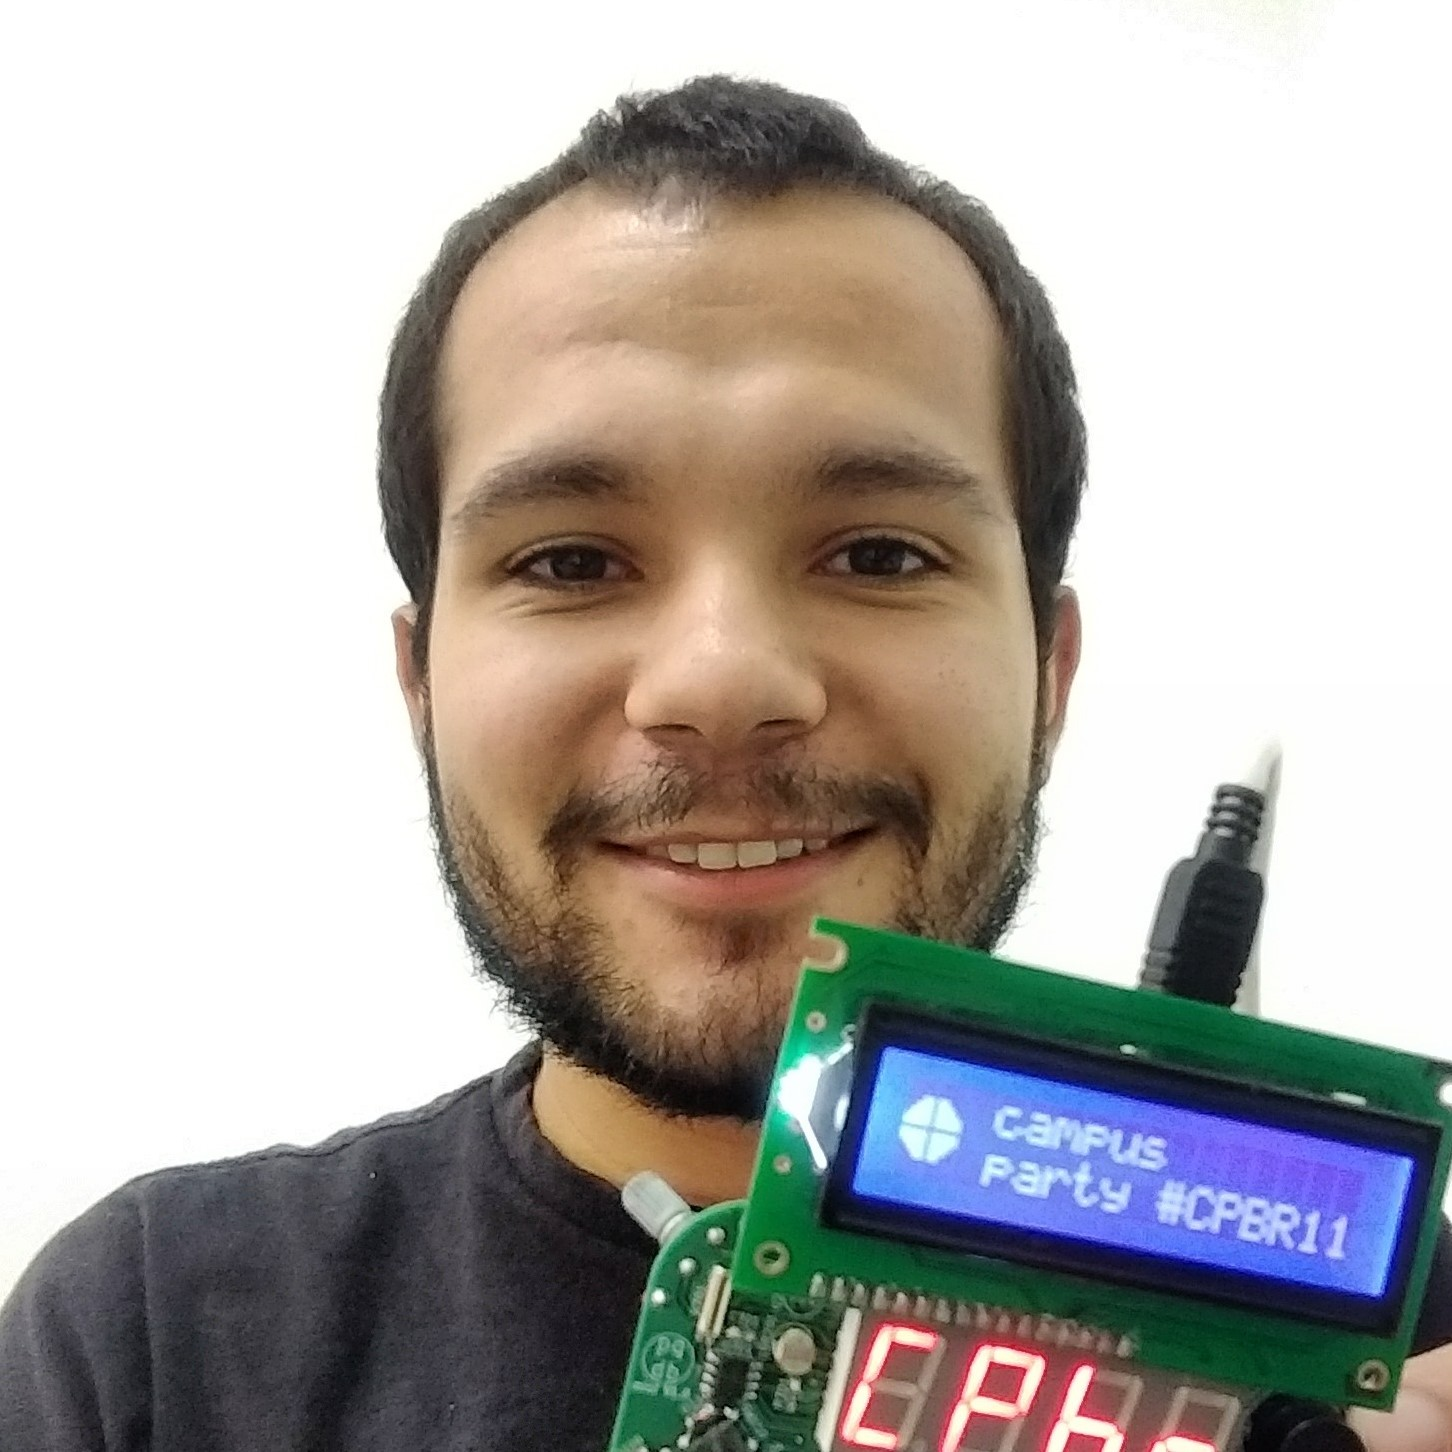
\includegraphics[width=4cm]{photo}
\section{Contato}
\href{https://wa.me/5511945545955}{(11) 94554-5955}
~
\href{mailto:rafaelmmoreira@gmail.com}{rafaelmmoreira@gmail.com}
~
\url{https://www.linkedin.com/in/rafaelmmoreira/}
~
\url{https://github.com/rafaelmmoreira/}
%
\section{Idiomas}
Português: nativo
Inglês: fluente
Espanhol: avançado
Francês: iniciante
%
\section{Interesses profissionais}
Desenvolvimento de software
Prototipagem de hardware
Análise de dados
Ensino e popularização de ciência e tecnologia
%
\vspace{3.7cm}
Veja a versão mais recente deste currículo

\includegraphics[width=4cm]{qrcode}
Available in English.
Disponible en Español.
%
\end{aside}

%----------------------------------------------------------------------------------------
%	SKILLS SECTION
%----------------------------------------------------------------------------------------

\section{Educação}
\vspace{-0.3cm}
\begin{entrylist}
\entry
{}
{\textbf{Mestrado em Ciência e Tecnologia da Computação}}
{}
{\textit{ Universidade Federal de Itajubá, 2019.}}
{}

\entry
{}
{\textbf{Graduação em Engenharia de Computação }}
{}
{\textit{ Universidade Federal de Itajubá, 2015.}}
{}

\entry
{}
{\textbf{Especialização em Data Science}}
{}
{\textit{Centro Universitário Faculdades Metropolitanas Unidas (em andamento).}}
{}

\entry
{}
{\textbf{Especialização em Desenvolvimento de Software com Metodologias Ágeis}}
{}
{\textit{Universidade Anhembi Morumbi (em andamento).}}
{}

\end{entrylist}
{\vspace{-0.8cm}}
%	WORK EXPERIENCE SECTION
%----------------------------------------------------------------------------------------

\section{Experiência}
\vspace{-0.3cm}
\begin{entrylist}
%------------------------------------------------


%----------------------------------------------------------------------------------------
\entry
{}
{Analista de Sistemas PL | Setis Automação e Sistemas (PayGo/C6 Bank) | out/18 - atual}
{\vspace{-0.01cm}}
{Desenvolvimento e manutenção de software embarcado para modelos variados de terminais POS ("maquininhas" de cartão) para uma adquirente de grande porte utilizando linguagem C e metodologia Scrum. Automação de processos de geração de pacotes utilizando Python.}
{}
 %----------------------------------------------------------------------------------------

\entry
  {}
  {Professor de programação | Let's Code Academy | jan/19 - atual}
  {\vspace{-0.01cm}}
{Professor do curso Python Pro (algoritmos, estruturas de dados, programação orientada a objeto, interface gráfica, consumo de APIs e webscraping). Produção de livro-texto completo para o curso Python Pro e de capítulos para o livro-texto de Data Science.}
 {} %----------------------------------------------------------------------------------------

\entry
  {}
  {Professor temporário | Universidade Federal de Itajubá | fev/17 - out/18}
{\vspace{-0.01cm}}
{ Professor de lógica de programação nos cursos de Engenharia de Computação, Eletrônica e de Controle e Automação. Linguagens C e Python. Coordenou os projetos Dev-U (equipe de desenvolvimento de jogos) e ProgramAção (grupo de professores de programação voluntários para adolescentes).}
 %----------------------------------------------------------------------------------------
\end{entrylist}
{\vspace{-0.4cm}}

\section{Palestras e treinamentos}
\vspace{-0.3cm}
\begin{entrylist}

\entry
{}
{Principais palestras e treinamentos ministrados em eventos técnicos:}
{}
{\vspace{-0.5cm}}

%------------------------------------------------
\entry
{}
{\href{https://www.slideshare.net/rafaelmmoreira/como-fazer-seu-prprio-gameboy-cpbr11}{Como Fazer Seu Próprio Gameboy}}
{\href{https://campuse.ro/events/campus-party-brasil-2018/workshop/como-fazer-seu-proprio-gameboy-cpbr11/}{Campus Party Brasil, 2018}}
{\vspace{-0.5cm}}
%------------------------------------------------
\entry
{}
{\href{https://www.slideshare.net/rafaelmmoreira/desenvolvimento-de-sistemas-embarcados-do-hardware-ao-software}{Desenvolvimento de Sistemas Embarcados}}
{\href{https://sp13.securitybsides.com.br/detalhe-dos-treinamentos-e-apresentacoes/}{BSides São Paulo, 2016}}
{\vspace{-0.5cm}}
%------------------------------------------------
\entry
{}
{\href{https://www.slideshare.net/rafaelmmoreira/escalonador-earliest-deadline-first-tdc2014sp}{Escalonador Earliest Deadline First}}
{\href{https://thedevconf.com/tdc/2014/saopaulo/trilha-embedded}{The Developer's Conference São Paulo, 2014}}
{\vspace{-0.5cm}}
%------------------------------------------------
\entry
{}
{\href{https://www.slideshare.net/rafaelmmoreira/programao-segura}{Programação Segura}}
{\href{https://garoa.net.br/wiki/O_Outro_Lado_BSidesSP_ed_naovaitercopa/Lightning_Talks}{BSides São Paulo, 2014}}
{\vspace{-0.5cm}}
%------------------------------------------------

%------------------------------------------------
\end{entrylist}
{\vspace{-0.2cm}}
%-------------------------------  ---------------------------------------------------------
%	END HOBBIES SECTION SECTION

\section{Publicações}
\vspace{-0.3cm}
\begin{entrylist}
%------------------------------------------------
\entry
{}
{}
{\vspace{-0.4cm}}
{\href{https://doi.org/10.1109/ICM48031.2019.9021277}{MOREIRA, R. M. et al. \textbf{Online Heartbeat Classification Using Low Cost Algorithms}. In: 31st INTERNATIONAL CONFERENCE ON MICROELECTRONICS (IEEE-ICM), 2019, Cairo, Egito.}}
{}
%------------------------------------------------
\entry
{}
{}
{\vspace{-0.01cm}}
{\href{http://www.swge.inf.br/CBA2014/anais/PDF/1569927865.pdf}{MOREIRA, R. M. et al. \textbf{Plataforma Didática de Baixo Custo para Experiências em Laboratórios de Controle}. In: XX CONGRESSO BRASILEIRO DE AUTOMÁTICA, 2014, Belo Horizonte.}}
{}
\end{entrylist}
{\vspace{-0.4cm}}

%%%%%%%%%
\section{Linguagens e tecnologias}
\vspace{-0.3cm}
\begin{entrylist}
\entry
{}
{Principais linguagens de programação}
{C, Python}
{\vspace{-0.5cm}}
\entry
{}
{Ferramentas de modelagem e análise de dados}
{Anaconda (Python), MATLAB, Octave}
{\vspace{-0.5cm}}
\entry
{}
{Microcontroladores e placas embarcadas}
{Arduino, Raspberry Pi, HCS12, PIC18F}
{\vspace{-0.5cm}}
\entry
{}
{Metodologias ágeis}
{Scrum, XP}
{\vspace{-0.5cm}}
\entry
{}
{Versionamento de software}
{GitHub}
{\vspace{-0.5cm}}
\entry
{}
{Graus variados de experiência com outras linguagens e tecnologias e facilidade para aprender. }
{}
{\vspace{-4.0cm}}
\end{entrylist}


\end{document}